\chapter{Introduction}

Measurements and troubleshooting are two important tasks that network engineers and administrators
carry out quite often. To be able to maintain network in healthy conditions engineers need to perform
monitoring of the network every now and then. But monitoring is not the only task. Engineers also 
need to troubleshoot the network quite often. For that matter, in this paragraphs that follow we discuss basic network
tools and techniques which can be used to measure and debug the network. 

\section{Questions}

In this section we enumerate research questions that we would like to 
answer in this report. We foresee at least three important questions
in this report. Namely those are: {\bf (i) What to measure in the enterprise networks? }
By answering this question we attempt to shed the light
on most important characteristics in the network traffic analysis. Be it
latency, throughput, goodput, error and loss rate, availability.
{\bf (ii) How to measure?} Here we would like to answer how to perform the network measurements.
For example, how to select vantage point, how to minimize the 
dataset, but still be able to grasp the most important characteristics of
the network. {\bf (iii) When to measure?} This question is also important for a number of reasons.
Selecting correct measurement period and correct duration of the measurements intervals
will have the important impact on the quality of the research outcome.

By answering these questions properly one can illuminate the performance of the 
networking infrastructure. Note, in this work we are considering only small networks, comprising 
10-100 devices. However, we believe that these questions are also applicable to larger
networks and more complicated topologies.

\chapter{Background}

This section consists of several important parts: First, we 
discuss main characteristics of the network; Second,
we describe various types of network topologies and device 
orchestrations; Third, we present various tools which are useful
in enterprise network measurements; Finally, we discuss most widely spread 
network protocols to watch out for in the enterprise 
network traffic.

\section{Basic network characteristics}

We believe that there are several key network characteristics: delay, jitter, throughput, goodput, error and loss rates.
All these metrics can be used to measure the performance of the networked systems. In the paragraphs that follow
we will describe these metrics and try to explain why they are so important.

{\it Delay } is the time it takes for the packet (on network layer) to reach the other communication side. Delay can be 
one way or two way, also called {\it round trip time}. The former one is hard to measure since the clocks on both sides
need to be synchronized. Technically, of course we can use sophisticated algorithms and packet trains to measure one way 
delay (for example, the reader can look at the RFC 7679~\cite{rfc7679}). But most of the time people rely on half of the RTT. This 
metric is less accurate since the packets can travel different paths and, hence, delays can be different. But yet this metric 
is quite common. For example, {\it ping} utility reports RTT as the measure of delay. We should note that delay impacts 
user experience greatly, and therefore, it is good to have links with low delays.

{\it Jitter} is yet another important metric and is widely spread across network engineers. Jitter is the variation of the 
delay, that is jitter shows how much the delay is varying throughout time. This metric is important because it can 
affect how the protocol timers are calculated. For example, if the jitter is high, the calculated timers can be 
inaccurate and, hence, the performance of such protocols can be undermined. Thus, the lower the jitter the better, in 
authors opinion, the performance of the networked devices. One easy way to compute jitter is to build the histogram 
of the network delays and compute the variance.

{\it Throughput} is also important and it captures how much data (including protocol headers and user payload) 
 can be delivered throughout network system in predefined time interval. Typically, the throughput is measured
in Kb/s, Mb/s and Gb/s. Obviously, the larger is the throughput the better network operates. Networks with large 
throughput can service larger number of clients. {\it Goodput} is the same as throughput, but excludes 
the control data from the calculations. In other words, packet header is excluded from the calculations and only 
user's payload is considered.

{\it Error rate} describes how often the packets arrive at the receiver with the corrupted bits. Most of the protocols
use notion of reliability (that is if the data is corrupted it is requested again) and, hence, high error rate can 
reduce the performance of such protocols considerably. It is therefore important for the network engineers to avoid
highly unstable links. Different media and operational environments have different error rates. For example, wireless
links often have grater error rate than wired and optical links. Also, different applications have different 
tolerance to errors. For example, Voice over IP and Video over IP require error rates to be low. Mail systems, on the 
other side, can tolerate high error rates, because the system works in the background and corrupted packets can be 
requested again.

{\it Loss rate} is the final metrics that we will cover. Loss occurs, for example, when intermediary routers 
drop the packet because of congestion or corruption of the packet. Once again, similar to error rates, sensitive 
applications do not operate well in lossy environments. Hence, typically, network engineers design systems so that
such applications will use links with little loss, while other traffic such as HTTP and SNMP protocols can use 
less expensive, but yet, lossy links. Typically, wireless links with weak signal, for example, have higher loss rates than fat wired and optical links.

There are also other characteristics that can be measured, for example, the reader can take a look at the 
congestion and some other. But we are not going to cover those in this report.

\section{Topologies}

There are several key topologies that are used in enterprises: mesh, star and hybrid. {\it Mesh} 
topology is such topology in which every network element is connected to every other network element. The links can be 
wired, wireless and pseudo links (if we are talking about overlays). Mesh can be full and partial.
In full mesh, obviously, every element is connected every other element in the network. Consider,
for example, personal area network in which all nodes are connected using wireless medium. 
Wired meshes are expensive, though, and are rarely used in modern deployments. Meshes are 
crucial, however, when availability is a must. In mesh, some nodes can fail, yet, the network
will remain alive and packets will be delivered, not to all, but some devices at least. A typical mesh network 
topology is shown in Figure~\ref{fig:mesh}.

\begin{figure}[!hbt]\centering
  \includegraphics[width=0.8\textwidth]{graphics/mesh.png}
  \caption{Mesh topology}
  \label{fig:mesh}
\end{figure}

{\it Star} topologies are cheaper and less fault tolerant. In star-like topology one node becomes
the root, while others connected to the root element and all the traffic flows through it. 
Oftentimes, redundant links are added to the topology to bring some level of tolerance to failures.
A typical star topology is shown in Figure~\ref{fig:star}. 

\begin{figure}[!hbt]\centering
  \includegraphics[width=0.8\textwidth]{graphics/star.png}
  \caption{Star topology}
  \label{fig:star}
\end{figure}


Finally, there are also hybrid topologies, such as {\it hub-and-spoke} networks. In this type of
networks spoke nodes are connected to hubs, while hubs form a full mesh between each other. Such
networks are cheaper than full mesh, but more fault tolerant than star topologies. A typical network
is shown in Figure~\ref{fig:hybrid}.

\begin{figure}[!hbt]\centering
  \includegraphics[width=0.8\textwidth]{graphics/hybrid.png}
  \caption{Hub-and-spoke topology}
  \label{fig:hybrid}
\end{figure}


\section{Tools}

Network engineers use wide variety of tools for measuring the permanence of the networks and in debugging tasks.
All tools can be categorized based on tasks they are meant to be used for, such as, measuring and troubleshooting.

{\it Measurement tasks:} to measure performance of the network a common set of tools includes ping utility, tcpping utility, traceroute utility, nc tool,
speedtest and iperf, snmp statistics reports by agents and direct queries. In the following paragraph we will describe these tools.

{\it Ping} utility is the most common tool to measure reachability of a host and measure the round trip times. The tool is based 
on the ICMP protocol which we will describe later. This tool is widely available in Linux, Windows, BSD and Unix operating 
systems.

{\it TCPing} is another common network tool to measure the reachability of the TCP port in the network. But the tool can be also used 
to measure the time to establish a TCP connection. To our best knowledge this tool is widely available for Windows OS without any 
charges.

{\it speedtest and iperf} utilities were primarily designed for measuring the bandwidth between two systems. The later one has
client and server implementations. This means that to measure the bandwidth (both UDP and TCP connections can be used) one needs
to start first the server with the -s flag, and only then run the client with -c flag.

{\it treceroute} is used often to trace the path the packet takes from host A to host B. The tool uses ICMP under the hood. 
Not only it is used to trace the reachability of the intermediate routers but it also reports the RTTs.

{\it netcat, or nc} is the tool that is available in Linux distributions and commonly used to send the commands to the server over UDP sockets.
It can be used to measure the bandwidth. For example, network administrators can send large enough binary package to the server and measure the 
time it takes for the transmission to happen.

And finally {\it SNMP} can be used to collect reports from agents about network performance. Such characteristics as bytes per second 
delivered by the network interface, ping RTT and many more can all be collected from network devices either with direct queries
or with the help of agents.

{\it Troubleshooting}. A set of tools available in this category are: nmap, tcpdump, Wireshark, nslookup, dig, iproute, and ifconfig. All these
tools are indispensable in analyzing and troubleshooting the network problems. It is essential for any network engineer to be acquainted 
and actively apply these tools. In the paragraphs that follows we will describe what every tool means, but briefly.

{\it nmap} is a tool that allows network engineer to detect open network ports (both UDP and TCP). Essentially, the tool scans the 
remote system and reports which port is open. Network engineers and hackers actively use this tool to detect weak points in the 
network systems.

{\it tcpdump and Wireshark}. These tools are helpful in collecting and analyzing network protocols. tcpdump is typically used
to collect the raw packets and frames from the network interface of interest, while Wireshark is more advanced: it can analyze the
network traffic and export it to XML and JSON file formats. We ourselves use these tools in our network traffic analysis tasks.

{\it nslookup and dig} are used to detect the problems with the DNS servers and queries. These tools are often used by network 
engineers to detect the problems with DNS and get information about remote systems. 

{\it iproute} is a tool that can be used for multiple purposes, but primarily these tools are useful in configuring the routes to remote 
systems. For example, network engineers can use the tool to check whether the routes to remote hosts exist. It can be also used to add
static routes. But these are just few examples. 

And finally, {\it ifconfig} tool can be used to configure the network interfaces. For example, network engineers can use this tool
to set default gateway, IP address on the interface, and set the DNS server IP address, either manually or with help of DHCP server.  
 
\section{Network protocols to watch out for}

There is humongous amount of protocols in modern networks: from L2 STP to Voice of IP at L4. But we are interetested in only 
few protocols that one should watch out during basic network analysis and troubleshooting: We will cover L2 STP protocol, TCP, UDP, ICMP, DNS, DHCP
and some security protocols at L4 such as SSH and TLS.

\subsection{Spanning trees}

Spanning tree protocol or STP is one of the most important protocols in local area networks. STP builds 
a tree without loops so that frames will not loop forever in the network. 

Spanning tree protocol operates on the L2 and is responsible for constructing the loop-free network topologies.
Recall, L2 frames do not have TTL fields like IP protocol. And so if the network is not loop-free the 
frames can circulate endlessly in the network. 

STP operates in phases. First, the network switches elect the so called root bridge - the bridge that 
will be the root of the tree. Switches do so by broadcasting their identifiers - the switch with the 
lowest identifier is elected as root. Once, the root switch is elected nodes start to construct the tree
by assigning  roles to the ports: the port can be either root port, designated port or blocked port.
The root bridge assigns all of its ports as designated ports. Other switches assign ports as
root ports if they have the shortest distance to the root bridge. The switch assigns the remaining ports as
designated ports if they are closer too root port on the segment. The remaining ports become 
blocked and so no traffic can traverse these ports. The initial implementation was defined in IEEE 802.1D
standard. Later more efficient protocols were defined for example consider Rapid STP, Per VLAN STP.
These protocols have faster convergence time and can be used to defined different spanning trees
for each VLAN.

\subsection{TCP, UDP and ICMP}

There are variety of the protocols on transport layer. But we are going to cover 
only three such protocols: TCP, UDP and ICMP.

TCP protocol is the transport layer protocol. Transmission control protocol, or TCP,
uses acknowledgments to deliver the packets in the network. In other words TCP is a 
reliable protocol, since unacknowledged packets are being sent again. Many application layer protocols
use TCP for transport. For example, SSH, HTTPS, FTP and other all use TCP as the base, since these
protocols do not tolerate packet losses. 

TCP session starts with 3-way handshakes. First the initiator, or client, sends SYN packet.
Upon reception of the SYN packet the server sends the SYN+ACK packet. And finally, the 
client acknowledges the reception of the SYN+ACK with ACK packet. During the handshake
the parties also exchange the initial sequence numbers between each other. The completion
of the communication session happens with two-way handshake. One party sends FIN packet 
and the other sends FIN+ACK packet.

TCP protocol requires two IP addresses and two ports. There exist well defined ports 
for common TCP applications. It is important to look for these well known ports during the 
traffic analysis. In Table~\ref{tab:tcpports} we list some of the well known TCP ports.

\begin{table*}[h!]
  \caption{Well-known TCP ports}
  \label{tab:tcpports}
  \centering
  \begin{tabular}{lc}
    \hline
    {\bf Protocol} & {\bf Ports }\\
    \hline
    FTP            & 20/21 \\
    SSH            & 22 \\
    Telnet         & 23 \\
    SMTP           & 25 \\
    DNS            & 53 \\
    HTTP           & 80 \\
    POP            & 110 \\
    IMAP           & 143 \\
    HTTPS          & 443 \\
    LDAP           & 389 \\
    \hline              
  \end{tabular}
\end{table*}

User Datagram protocol or UDP does not guarantee reliable delivery of the packets.
So, typically it is used together with such protocols as VoIP, Dynamic Host Configuration Protocol (DHCP).
And redundancy is typically embedded into the UDP protocol by the upper layer protocols. And in case
of loss or corruption, upper layer protocols use this redundancy to mask these failures.
UDP, however, similarly to TCP protocol uses port numbers to make the connections. 
Retransmissions are also controlled by the application itself.

Most important UDP protocols and ports are shown in Table~\ref{tab:udp}.

\begin{table*}[h!]
  \caption{Well-known TCP ports}
  \label{tab:udp}
  \centering
  \begin{tabular}{lc}
    \hline
    {\bf Protocol} & {\bf Ports }\\
    \hline
    DNS            & 53 \\
    DHCP           & 67/68 \\
    SNMP           & 161 \\
    TFTP           & 69 \\
    RTP            & dynamic \\
    NTP            & 123 \\
    SIP            & 5060 \\
    QUIC           & 443 \\
    \hline
  \end{tabular}
\end{table*}

Internet Control Message Protocol is typically used to detect liveness of the hosts in the Internet,
as well as to send error messages to the sender. ICMP used in such utilities as ping and traceroute.

\subsection{DNS and DHCP}

DNS protocol or Domain Name Service protocol is used to resolve fully qualified domain name
(FQDN) into IPv4 and IPv6 addresses. It is also used to perform reverse transformation from
IP address to domain name. DNS is vital in modern network as it allows not to remember the IP
address of the system, but, instead, human readable name of the resource.

DNS resolver works recursively: At first, host sends the query to designated DNS server (typically
the same machine as the default router or a dedicated DNS server); Second, DNS server sends 
the query to the top level domain (TLD); TLD responds with the root server IP responsible for
the name in the query, and DNS server sends next query to root DNS server; Finally, the DNS server sends
the query to target DNS server and resolves the FQDN into IPv4 or IPv6 address.

Dynamic Host Configuration Protocol is a handy protocol that allows configuring hosts
with IP address (both IPv4 and IPv6 versions exist), default gateway, DNS server 
and other parameters. DHCPv4 operates in 4 phases (or 4-way handshake). First,
the client send DISCOVER packet (broadcast) seeking for the DHCP server. DHCP server
responds with the OFFER (it offers IP address). Later on the client, if it accepts the 
IP address sends DHCP REQUEST packet in unicast fashion. And finally, the server responds
with ACK packet. After such configuration the client can communicate with the rest 
of the network elements in the network. There is also DHCPv6, but it is used for configuration
of the IPv6-enabled clients. The operation is quite similar to IPv4 version.

\subsection{LDAP and other Windows services}

There are several key Windows protocols that you will typically see in the network. LDAP, Kerboros
and WINS are just few examples.

The Lightweight Directory Access Protocol (LDAP) is an open, vendor-neutral application 
protocol for accessing and maintaining distributed directory information services (like user 
accounts, passwords, and network resources) over an IP network. LDAP often operates on TCP port
389.

The WINS (Windows Internet Name Service) protocol is a legacy Microsoft service that dynamically maps 
NetBIOS names (like COMPUTERNAME) to IP addresses (similar to DNS protocol), acting as a centralized, dynamic phonebook for older Windows networks, 
reducing reliance on noisy network broadcasts for name resolution. 

\subsection{What about timing: NTP}

Keeping time synchronized in the network is important. Many applications rely on accurate timing.
For example, application logging system puts the timestamps in the files, precise activation of scheduled jobs relies on 
system time, and so on.

NTP was defined in RFC 5905~\cite{rfc5905} and is commonly used by network devices to synchronize clocks.
NTP operates on UDP port 123, so it is important that firewall will allow this port to be open.

\subsection{SSH, TLS and other security protocols}
	
There is large body of security protocols. Examples are: HIP, TLS, SSL, SSH, IKE, IPsec and many, many more.

Secure socket layer (SSL)~\cite{ssl} and Transport Layer Security (TLS)~\cite{tls} are an application
layer solutions to secure TCP connections. SSL was standardized in RFC 6101.
TLS was standardized in RFC 5246. And was designed to prevent eavesdropping,
man-in-the-middle attacks, tampering, and message forgery. In SSL communicating
hosts can authenticate each other with the help of longer-term identities - public key certificates.
SSL is great for building VPN tunnels and protecting upper-layer protocols such as HTTP.

Secure Shell protocol (SSH) is the application layer protocol that provides an encrypted channel
for insecure networks. SSH was originally designed to provide secure remote command-line, login,
and command execution. But in fact, any network service can be secured with SSH. Moreover, SSH
provides a means for creating VPN tunnels between spatially separated networks: SSH is a great
protocol for forwarding local traffic through remote servers.

There are other security protocols (actually, quite a log). For example, Host Identity Protocol. 
Thus, internet was designed initially so that the Internet Protocol (IP) address has a dual role: it
is the locator, so that the routers can find the recipient of a message, and it is an identifier
so that the upper layer protocols (such as TCP and UDP) can make bindings (for example, transport
layer sockets use IP addresses and ports to make connections). This becomes a problem when a networked
device roams from one network to another, and so the IP address changes, leading to failures in
upper-layer connections. The other problem is the establishment of an authenticated channel between
the communicating parties. In practice, when making connections, the long-term identities of the parties
are not verified. Of course, solutions such as SSL can readily solve the problem at hand. However, SSL
is suitable only for TCP connections, and most of the time, practical use cases include only secure web
surfing and the establishment of VPN tunnels. Host Identity Protocol, on the other hand, is more flexible:
it allows peers to create authenticated secure channels on the network layer, so all upper-layer protocols
can benefit from such channels. More on the protocol can be found in~\cite{gurtov:hip}.

HIP relies on the 4-way handshake to establish an authenticated session. During the handshake, the
peers authenticate each other using long-term public keys and derive session keys using Diffie-Hellman
or Elliptic Curve (EC) Diffie-Hellman algorithms. To combat the denial-of-service attacks, HIP also
introduces computational puzzles.

HIP uses a truncated hash of the public key as an identifier in the form of an IPv6 address and
exposes this identifier to the upper layer protocols so that applications can make regular
connections (for example, applications can open regular TCP or UDP socket connections). At the
same time, HIP uses regular IP addresses (both IPv4 and IPv6 are supported) for routing purposes.
Thus, when the attachment of a host changes (and so does the IP address used for routing purposes),
the identifier, which is exposed to the applications, stays the same. HIP uses a particular
signaling routine to notify the corresponding peer about the locator change. More information
about HIP can be found in RFC 7401~\cite{rfc7401}.

\subsection{Watch out for anti-virus}

Upon examination of the logs we have observed that quite a lot of connections were made 
to the anti-virus server. This protocol consumes a lot of bandwidth and seems to be 
vital in modern enterprise networks. In Table~\ref{tab:apps} we can see that 
anti-virus applications sends more packets than any other network applications in the system.
The bottom line is the following: not only anti-virus is important in the network and needs to
be installed on all the computers, but also the signature database need to be up-to-date.

\chapter{Results}

Analyzing the traffic in the company on regular basis can be 
benficial for several reasons: (i) we can find strange behaviour 
of computers in the network, (ii) we can find the bottlenecks, 
(iii) we can detect misconfigurations in networked devices. 
In the paragraphs that follow we present the analysis traffic 
which was captured in a small enterprise network. 

\section{Data collection}

We begin this section with a description of the enterprise network,
with the details of data capturing process to follow. According to 
Cisco documentation~\cite{cisco:ccent}, our network was two-tier 
medium-sized enterprise network comprising slightly more than 
$200$ workstations, one distribution switch (Cisco Catalyst 
G3560 series layer 3 switch), one router (the router was 
running Linux operating system) playing the role of a 
{\em VLAN router}, $6$ access switches from various vendors (1 DLink DES3200, 
1 Cisco 2690, 2 DLink DES1226 and 2 XNET SH9024 switches)
and also multiple, non-managed switches and one wireless 
access point all being connected to access switches.

\begin{figure}[h!]
\centering
\includegraphics[width=0.4\textwidth]{graphics/network_arch.png}
\caption{Enterprise network architecture}
\label{fig:network}
\end{figure}

Since we were unable to analyze fully the wiring of the access (especially those that were spread around the building and connected 
directly to access switches) and distribution switches, we could basically only guess (based on the limited information we had at our 
disposal) that there were no redundant links between access and distribution switches, also there were no redundant links between 
distribution switch and VLAN router. Essentially, the switches were merely connected in a tree like topology: each access switch was connected 
to one distribution switch, and the distribution switch was connected to a single router over a gigabit Ethernet trunk link. 

The entire network was partitioned into $25$ broadcast domains (VLANs), with native VLAN (VLAN that does not have tagging) being reserved 
for infrastructure management, although not all the switches were using native VLAN for management purposes. For brevity and privacy reasons 
we omit the discussion of network addressing in full detail, but rather mention that all VLANs were assigned addresses from class C private network from 
192.168.0.0 to 192.168.24.0, whereas the last usable address in each subnetwork was used as the address for the default gateway. 
All hosts in the network used static address assignment schema.

To capture the traffic it was natural to place packet capturing at 
the central router, rather than installing it on multiple 
switches. With this respect, we configured sniffer at the 
router to capture the frames on a gigabit trunk interface.
We have used {\em tcpdump} to capture all traffic on the trunk 
link of a router - the link which was connected to 
the distribution switch. The data collection period 
lasted for slightly more than $2.5$ hours, from 
$06:23$ UTC to $09:03$ UTC and $19.1 \cdot 10^6$ 
frames were collected in total. Of course, this is not enough
for the full picture (in practice the traffic needs to be collected for 
at least one week, but this interval was sufficient to 
understand what kind of traffic existed in the network). Once the data was 
collected, a single {\em pcap} file was created. 
We then started to preprocess the captured data.

\section{Breakdown of the network protocols in small enterprise network}

\begin{table*}[h!]
  \caption{Distribution of non IPv4 frames}
  \label{tab:non:ipv4:frames}
  \centering
  \scriptsize
  \begin{tabular}{lcc}
    \hline
    {\bf Protocol}                                   & {\bf Number of frames } & {\bf Fraction (\%)} \\
    \hline
    ARP                                              & 136857                  & 48.8 \\
    Cisco Shared Spanning Tree Protocol              & 119385                  & 42.5 \\    
    IPv6                                             & 17034                   & 6.1  \\
    Spanning Tree Protocol (IEEE 802.1D)             & 4774                    & 1.7  \\
    IPX                                              & 1164                    & 0.4  \\
    Cisco Loop                                       & 957                     & 0.3  \\
    Cisco CDP/VTP                                    & 510                     & 0.2  \\
  \end{tabular}
\end{table*}



To perform the preprocessing we have extracted the binary data
and stored it in {\em pdml} (Packet Description Markup Language) 
format - a special XML format which is used to describe the 
contents of the binary representation of frames and packets.

Our next step was to extract needed fields from the XML 
file and store the extracted data in the format which was 
simpler for further analysis. Thus, we have chosen 
JSON (JavaScript Object Notation) format. From PDML
we have extracted the following fields:

\bi
  \im Ethernet source and destination MAC addresses and type field
  \im VLAN identifier and type field
  \im From IP header we have extracted source and destination 
      addresses, version number, length, protocol type, and TTL.
  \im Basic information from GRE and PPP headers (since 
      clients accessing the Internet were using these protocols)
  \im From TCP header we have selected source and destination ports, 
      stream identifier, length, sequence and acknowledgment numbers, 
      as well as flags and window size.
  \im From UDP header source and destination ports, as well as datagram 
      length information were extracted.
\ei

Our next step in preprocessing the data was to extract non IPv4 frames - 
frames for which neither Ethernet type nor VLAN type field were equal to 
{\bf 0x00008000} (this dataset includes packets from all VLANs as well as
packets from native VLAN). Once the data was extracted we binned the 
frames according to protocol types. In Table~\ref{tab:non:ipv4:frames} 
we present the summary results for this data.


\begin{table*}[h!]
  \caption{Distribution of protocols in native VLAN}
  \label{tab:native:vlan}
  \centering
  \scriptsize
  \begin{tabular}{lcc}
    \hline
    {\bf Protocol}                                   & {\bf Number of frames } & {\bf Fraction (\%)} \\
    \hline
    Cisco Shared Spanning Tree Protocol              & 4774                    & 40.5 \\
    Spanning Tree Protocol (IEEE 802.1D)             & 4774                    & 40.5 \\
    Cisco Loop protocol                              & 957                     & 8.1  \\
    IP (ICMP only)                                   & 640                     & 5.4  \\
    Cisco CDP/VTP                                    & 510                     & 4.3  \\
    ARP                                              & 128                     & 1.1  \\
  \end{tabular}
\end{table*}

\begin{table*}[h!]
  \caption{Frames with invalid MAC addresses}
  \label{tab:invalid:mac}
  \centering
  \scriptsize
  \begin{tabular}{ccccc}
    \hline
    {\bf Source MAC}       & {\bf Destination MAC }        & {\bf Source IP}        & {\bf Destination IP} &  {\bf Manufacturer}     \\ 
    \hline
30:f9:ed:41:a6:01 & 00:c0:ee:9a:5a:85 & 192.168.5.10 & 192.168.5.151 & Sony/KYOCERA \\
00:30:05:c2:b7:ff & 00:17:c8:03:a0:7b & 192.168.18.7 & 192.168.18.34 & Fujitsu/KYOCERA \\
00:15:58:67:5f:14 & 00:c0:ee:9a:5a:85 & 192.168.5.3 & 192.168.5.151 & FOXCONN/KYOCERA \\
    \hline
  \end{tabular}
\end{table*}



The next step in preprocessing of the data was to exclude the frames 
for the native VLAN from the traces. Thus, we have filtered out 
the frames for which Ethernet type was not equal to {\bf 0x00008100}.
It turned out that the fraction of frames without VLAN tag was rather 
small and constituted only $0.06 \%$ of the total number of frames in 
the trace. Since native VLAN was used only for management purposes
we excluded it from further analysis. However, in Table~\ref{tab:native:vlan} we show 
the  distribution of packet types seen in the native VLAN.

\begin{table*}[h!]
  \caption{Distribution of top applications used in the network}
  \label{tab:apps}
  \centering
  \scriptsize
  \begin{tabular}{cccccc}
    \hline
    {\bf TCP port} & {\bf Frequency } & {\bf Application} & {\bf UDP port} & {\bf Frequency} & {\bf Application}       \\
    \hline
         13000     & 11599            &  Kaspersky        &        53      &      27960      & DNS                     \\
         443       & 10128            &  HTTPS            &        137     &      6589       & NetBIOS                 \\
          88       & 9700             &  Kerboros         &       389      &      1350       & LDAP                    \\
          80       & 6938             &  HTTP             &     15000      &      804        & Kaspersky Network Agent \\
          445      & 5581             &  Microsoft SMB    &        88      &      166        & Kerboros                \\
          135      & 940              &  MS RPC           &       123      &      146        & NTP                     \\
          389      & 880              &  LDAP             &      13000     &      50         & Kaspersky               \\
          49155    & 694              &  Microsoft-DC     &      138       &      21         & NetBIOS                 \\
          139      & 682              &  Netbios          &      443       &      16         & QUIC                    \\
    \hline
  \end{tabular}
\end{table*}

Instead, next we turned our attention to frames with invalid MAC addresses. 
By invalid MAC address we mean those MAC addresses which are not multicast or 
broadcast addresses received at the trunk interface of the router with 
destination unicast MAC addresses not of router's own MAC addresses. 
Upon filtering the data we have found that there were two such 
destination unicast MAC addresses. We hypothesize that such frames could have been
received at the trunking interface due to the following reasons. The MAC
address table of the switches (i) did not contain a record for the destination 
MAC address and so it was flooded to all ports except the port from which 
the frame was received; (ii) wrong mapping for the destination MAC 
address and outgoing interfaces could have existed and so it was 
forwarded into the wrong port of the switch and thus was received at the 
trunk port of the router. The two invalid MAC addresses we have discovered are: 
{\bf 00:17:c8:03:a0:7b} and {\bf 00:c0:ee:9a:5a:85}. We leave this 
investigation to the network administrators.


Our next step of data preprocessing was to find for every packet being 
forwarded a corresponding pair: Note, our trace contained two copies 
of a packet for which the source and destination IP addresses where within 
the {\em 192.168.0.0/16} subnetwork with a difference that TTL was reduced 
by one for one of the packets, and the Ethernet header was recalculated. 
Thus, by filtering out the duplicates we were able to excluded the 
possibility of overcounting the number of bytes carried in TCP and 
UDP streams, and other transport protocols. To perform this filtering step, 
we merely found all packets whose source and destination addresses where within 
the subnetwork {\em 192.168.0.0/16} and filtered out frames for which 
source MAC address was not equal to the MAC address of the VLAN server
(note, all VLAN interfaces were assigned the same MAC address). 
Thus, effectively leaving only one copy of the packet being forwarded 
between the subnetworks in the trace. Our resulting trace was reduced by
$35.4 \%$, and now contained $12190001$ frames.

Once again we have searched for frames with invalid MAC
addresses (we have introduced the term invalid MAC addresses in the
previous paragraphs). In Table~\ref{tab:invalid:mac} we list these
MAC addresses as well as corresponding IP addresses found in such
frames, and manufacture's name. Obviously, such disripancy is strange.



\begin{figure}[!hbt]\centering
  \includegraphics[width=0.9\textwidth]{graphics/interaction_between_local_computers_over_tcp.pdf}
  \caption{Interaction between computers in different VLANs over TCP}
  \label{fig:interaction}
\end{figure}

\begin{figure}[!hbt]\centering
  \includegraphics[width=0.9\textwidth]{graphics/distribution_of_frame_sizes.pdf}
  \caption{Distribution of frame sizes}
  \label{fig:frame_sizes}
\end{figure}

For the cleaned data, our first step was to take a look at the distribution of TCP and UDP applications and the number of bytes these 
applications transmitted. Thus, in Table~\ref{tab:apps} we show the distribution of $9$ most used UDP and TCP applications. We examened 
both inter-VLAN and Internet traffic. We observed that while most of hosts were not actively connected to the Internet, using the VPN 
connections, $15366$ connection attemps were made towards the Internet (only TCP SYN packet was captured, which was dropped by the 
firewall). This could be an indication that quite a lot of connections are made in fact in a stealth mode on users' computers. 

\begin{figure}[!hbt]
  \includegraphics[width=0.9\textwidth]{graphics/bubble_plot_distribution_of_open_ports.pdf }
  \caption{Distribution of ports used in the network}
  \label{fig:ports}
\end{figure}   

Next we computed the distribution of the packet sizes for packets with valid IP addresses. Interestingly there were frames which were larger than maximum allowed Ethernet frames 
size (so called jumbo frames). Around $10\%$ of the IPv4 packet were larger than $1500$ bytes. In Figure~\ref{fig:frame_sizes} we show this distribution.


To finilize the discussion, we have also plotted the distribution of port and IP addresses. In Figure~\ref{fig:ports} we show this distribution.


\section{Watch out! We are plotting the network map}

Next, we have computed the adjacency graph for computers which were interacting over TCP in the local network (an interaction here means that at 
least one TCP/UDP connection between the pair of computers existed). \eat{In Figure~\ref{fig:interaction} we demonstrated the graph of 
interaction for TCP connections only.} As it was expected, only few computers (servers) were accepting all TCP connections, with a small 
fraction of computers were interacting between each other. Upon expecting closely the logs we have found few interesting things: (i) at 
least one machine had misconfigured address (it was using self generated IP addresses with the prefix $169.254.171.0/24$); (ii) 
only two machines were interacting with non-server computers $192.168.23.13$ and $192.168.3.6$ using ports $139$ and $445$.


\section{Performance, performance and once again performance: Stressing the network}

We have also stress-tested the network on ragular bases. For example, we have tested the bandwidth
between the gateway and the host in the Internet in order to udnerstand the performance of the outside
network. In addition it is important to measure the performance of the links between hosts and servers.
All this is done with the monitoring software.

\section{VPN connections}

Finally, we have monitored the  long-living VPN connections. Upon doing so, we have noticed that 
service providers do not play nicely with such connections.
For example, we have observed that TCP connections can enter so called 
{\it stale} state: ACKs do not go through in both directions,
but only one. In this case, the connection remains in 
ESTABLISHED state, but the data does not go through.
The result of the sequence progress is shown in Figure~\ref{fig:tcp}.

\begin{figure}[h]
\centering
\includegraphics[width=0.9\textwidth]{graphics/sequence_progress.pdf}
\caption{TCP sequence progress in both directions}
\label{fig:tcp}
\end{figure}

Clearly, drop of the spikes indicate TCP connection restarts. But one thing
is really interesting, the last TCP connection restarts successfully, but the sequences
are progressing only for one direction: from client to server. The data does not go 
through the CGN from server to client and the TCP connection hangs.

\chapter{Conclusions}

In this short report we have played a bit with the packets which were captured in a small enterprise. Our primary goal was to analyse the
interactions of computers and build the statistics for the traffic which was captured for several hours. Our key findings are 
the following: (i) major traffic in the network is HTTPS and HTTP, (ii) antivirus solutions consume considerable amount of 
bandwidth, (iii) computers in the network mainly interact with the default gateway and few servers, such as NFS server and mail server.

